\documentclass [../article.tex]{subfiles}
\begin{document}
  \section{Patterns in Data}
  A real world application of Fourier Transform is when
  looking for patterns within what looks like useless or
  confusing data. 
  \subsection{Example: Uncertain Principles}
  In his blog Chad Orzel explained this use
  case to his readers. He gathered the daily traffic data on his
  blog for the past one thousand and twenty-four days, the closest
  power of two to three years to make the transform work nicer.
  \begin{figure}[htbp]
    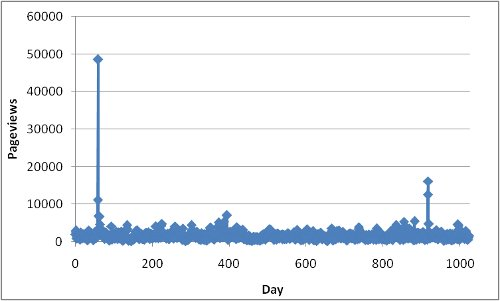
\includegraphics[width=\linewidth]{evar/1.jpg}
    \caption{Views Per Day.}
    \label{fig:views}
  \end{figure}
  Figure~\ref{fig:views} showcases this data, however from the
  graph it is hard to discern any pattern except for those two peaks 
  when there were popular blog post published. 
  From just looking at this graph
  alone and doing nothing else with it we do not learn much
  about the traffic. So we apply Fourier Transform to this
  data set to get Figure~\ref{fig:viewfreq}.
  \begin{figure}[htbp]
    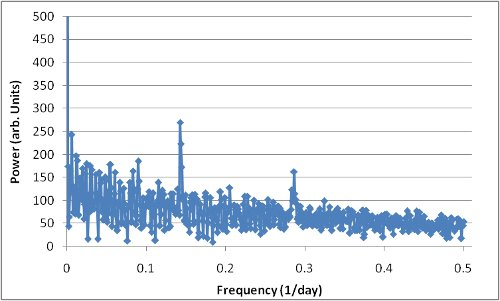
\includegraphics[width=\linewidth]{evar/2.jpg}
    \caption{View Frequency Spectrum.}
    \label{fig:viewfreq}
  \end{figure}
  This graph shows us how much power a certain frequency has over
  the original data set. As you can see there are two relatively 
  larger spikes in the graph excluding the one at ``0'' as that is 
  another aspect of Fourier Transformation. These two spikes indicate
  that those frequencies are quite powerful in our data series and thus
  point towards a possible pattern.
  \begin{figure}[htbp]
    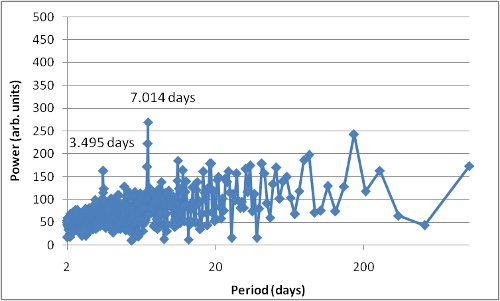
\includegraphics[width=\linewidth]{evar/3.jpg}
    \caption{View Period Strength.}
    \label{fig:viewperiods}
  \end{figure}
  To convert frequency to a time period the reciprocal was taken and then
  put on a log scale to highlight the pattern more clearly. From this graph 
  we see that through Fourier Transformation we can notice that a very
  strong recurring pattern is occurring every week as well as a
  smaller one every half week. Due to the fact that he only sampled
  at the end of the day we can not see any frequency faster than one
  day. Thus there could be a pattern of people reading in the evening as 
  apposed to the morning that we just can not see.
  \begin{figure}[htbp]
    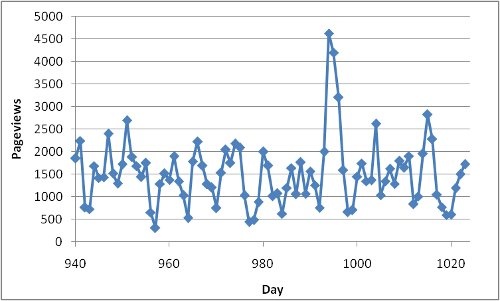
\includegraphics[width=\linewidth]{evar/4.jpg}
    \caption{Views Per Day Closeup}
    \label{fig:viewcloseup}
  \end{figure}
  If we zoom in on our first graph we can see this representation very
  well. Every seven days there is a strong dip downwards  which is
  why in the Fourier Transform graph there is a large appearance of
  a certain sin wave as well as the impact of the smaller wave every
  half week.
  \subsection{Example: Supplyframe}
  In another example we are going to look at data over a certain
  amount of time, much like we did in the previous example. 
  Greg Lin recorded the total number of
  user actions on his website over the course of multiple days. 
  By looking at Figure~\ref{fig:useractions}
  \begin{figure}[htbp]
    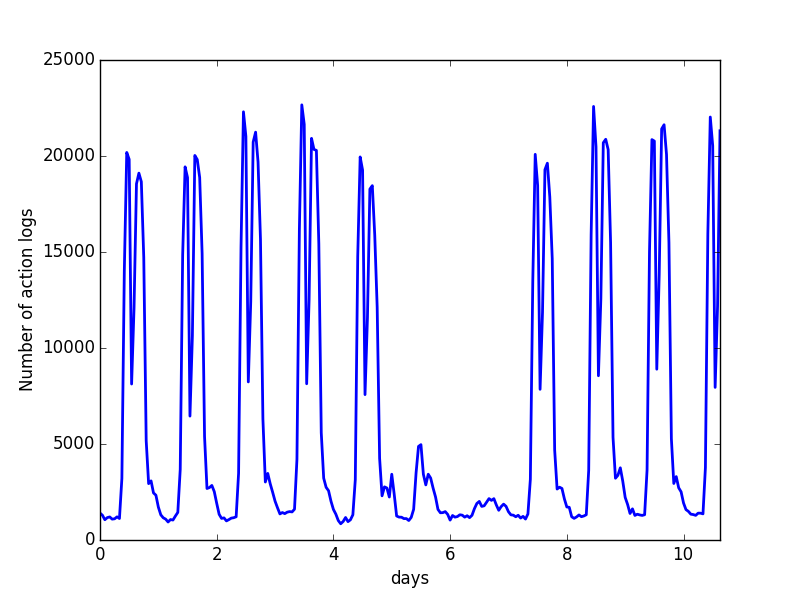
\includegraphics[width=\linewidth]{evar/5.png}
    \caption{User Actions.}
    \label{fig:useractions}
  \end{figure}
  we are able to easily identify a periodic pattern in
  the graph. Is there anything else that we may be missing, and
  how would we quantify these patterns?
  Perhaps there is something we can not see, so we apply the
  Fourier Transform to the set.
  \begin{figure}[htbp]
    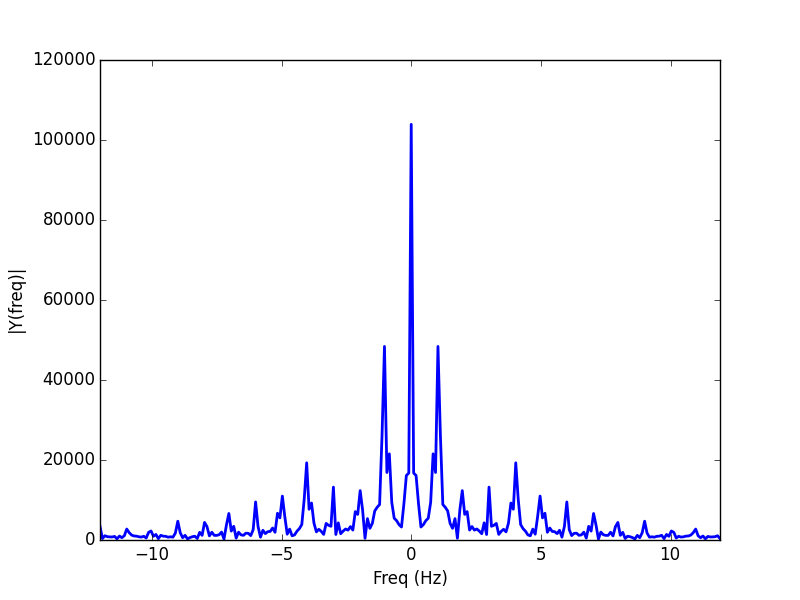
\includegraphics[width=\linewidth]{evar/6.png}
    \caption{User Action Spectrum.}
    \label{fig:actionspectrum}
  \end{figure}
  In Figure~\ref{fig:actionspectrum} we notice that most of the actions 
  on the site are using a low frequency sin wave. Now that the Fourier 
  Transform is available we can directly compare the frequencies of the 
  components to those of the original graph.
  \begin{figure}[htbp]
    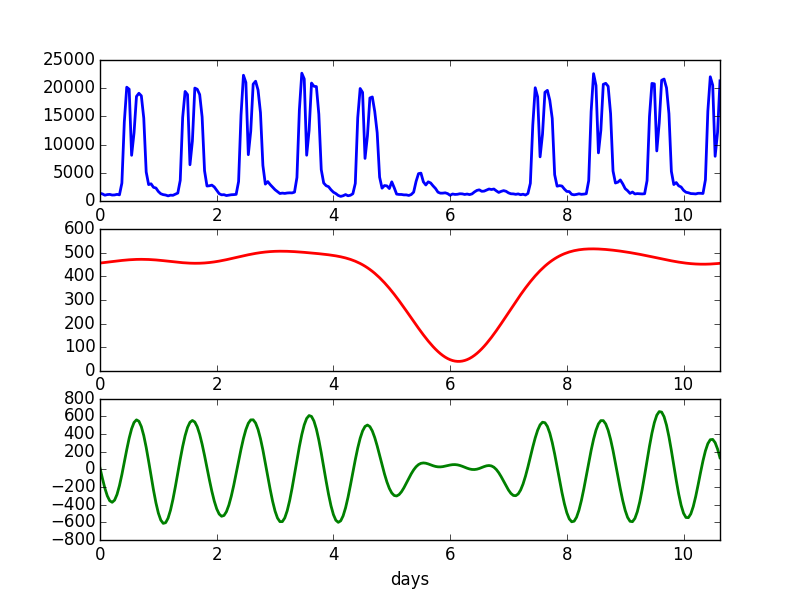
\includegraphics[width=\linewidth]{evar/7.png}
    \caption{I don't know.}
    \label{fig:idk}
  \end{figure}
  The second graph in Figure~\ref{fig:idk} is the components of the
  transform with frequency less than $|.46|$ and under that is
  components with frequency between $|.46|$ and $|1.40|$.  The author
  notes that  the graph with the red line really shows how on
  weekends the amount of actions is extremely low and how the
  green graph shows how nice and fluid the dip is that represents
  when people are working and when they are not. We get a clear
  understanding of what exactly is going on if it it were possible
  to have access to more graph and at more frequencies we would be
  able to exactly replicate the original graph.

  With the Fourier Transform we are able to see patterns we may not 
  have been able to see before and allows us to better
  understand it. With this technique people are able to
  base their programs and experiments with much better evidence
  and data.
\end{document}
